% Plane graph of the omnitruncated 3-cube (truncated cuboctahedron).
% Each vertex is labeled by its own coordinate vector x = x1 x2 x3,
% a signed permutation of 123 (a bar over position i means x_i < 0).
%   Purple hexagons  <-> vertices of the cube:  fixed sign vector (bar pattern by POSITION)
%   Blue   squares   <-> edges of the cube:     the two entries of magnitude 2,3 sit in
%                                               two fixed positions with fixed signs
%   Green  octagons  <-> facets of the cube:    the entry +-3 sits in a fixed position
%                                               with fixed sign; x3 = -3 is the outer face.
% Two vertices are adjacent iff they differ by swapping the magnitudes k,k+1 in place
% (signs stay with the positions) or by flipping the sign of the entry +-1.
% Requires: \usepackage[dvipsnames]{xcolor}, \usepackage{tikz}
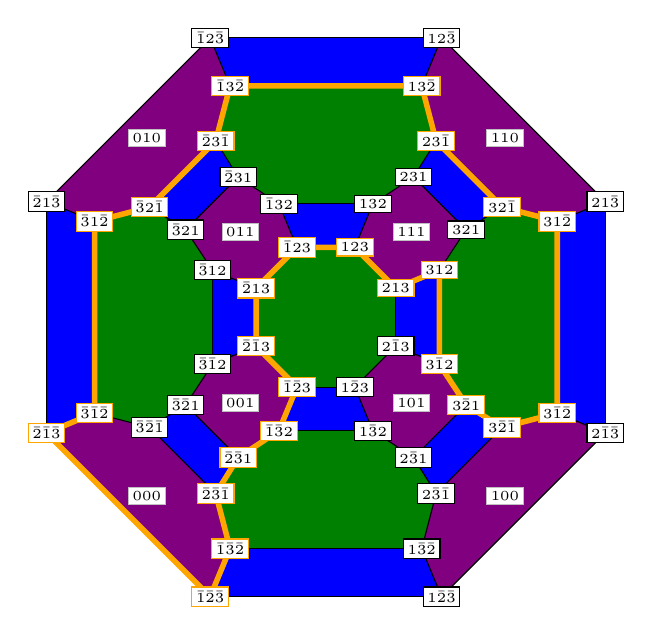
\begin{tikzpicture}[scale=1.2, every node/.style={font=\tiny, inner sep=1.5pt}]

% radii of the six concentric rings (= levels x3 = 3,2,1,-1,-2,-3)
\def\rA{0.80}\def\rB{1.30}\def\rC{1.75}\def\rD{2.20}\def\rE{2.65}\def\rF{3.20}

% ring 1: octagon of the facet x3 = +1  (vertices with x3 = 3)
\foreach \n/\a in {213/22.5, 123/67.5, n123/112.5, n213/157.5,
                   n2n13/202.5, n1n23/247.5, 1n23/292.5, 2n13/337.5}
  \coordinate (\n) at (\a:\rA);
% ring 2: vertices with x3 = 2
\foreach \n/\a in {312/22.5, 132/67.5, n132/112.5, n312/157.5,
                   n3n12/202.5, n1n32/247.5, 1n32/292.5, 3n12/337.5}
  \coordinate (\n) at (\a:\rB);
% ring 3: vertices with x3 = 1
\foreach \n/\a in {321/32, 231/58, n231/122, n321/148,
                   n3n21/212, n2n31/238, 2n31/302, 3n21/328}
  \coordinate (\n) at (\a:\rC);
% ring 4: vertices with x3 = -1
\foreach \n/\a in {32n1/32, 23n1/58, n23n1/122, n32n1/148,
                   n3n2n1/212, n2n3n1/238, 2n3n1/302, 3n2n1/328}
  \coordinate (\n) at (\a:\rD);
% ring 5: vertices with x3 = -2
\foreach \n/\a in {31n2/22.5, 13n2/67.5, n13n2/112.5, n31n2/157.5,
                   n3n1n2/202.5, n1n3n2/247.5, 1n3n2/292.5, 3n1n2/337.5}
  \coordinate (\n) at (\a:\rE);
% ring 6: octagon of the facet x3 = -1 (vertices with x3 = -3), the outer face
\foreach \n/\a in {21n3/22.5, 12n3/67.5, n12n3/112.5, n21n3/157.5,
                   n2n1n3/202.5, n1n2n3/247.5, 1n2n3/292.5, 2n1n3/337.5}
  \coordinate (\n) at (\a:\rF);

% vertices of the cube: hexagons (fixed bar pattern)
\foreach \pa/\pb/\pc/\pd/\pe/\pf in {
  213/123/132/231/321/312,
  n123/n213/n312/n321/n231/n132,
  n2n13/n1n23/n1n32/n2n31/n3n21/n3n12,
  1n23/1n32/2n31/3n21/3n12/2n13,
  21n3/12n3/13n2/23n1/32n1/31n2,
  n12n3/n21n3/n31n2/n32n1/n23n1/n13n2,
  n2n1n3/n1n2n3/n1n3n2/n2n3n1/n3n2n1/n3n1n2,
  1n2n3/2n1n3/3n1n2/3n2n1/2n3n1/1n3n2}
{
  \fill[Purple] (\pa) -- (\pb) -- (\pc) -- (\pd) -- (\pe) -- (\pf) -- cycle;
}
% edges of the cube: squares
\foreach \pa/\pb/\pc/\pd in {
  213/312/3n12/2n13,
  123/132/n132/n123,
  n213/n312/n3n12/n2n13,
  1n23/1n32/n1n32/n1n23,
  321/231/23n1/32n1,
  n231/n321/n32n1/n23n1,
  n3n21/n2n31/n2n3n1/n3n2n1,
  2n31/3n21/3n2n1/2n3n1,
  21n3/31n2/3n1n2/2n1n3,
  12n3/13n2/n13n2/n12n3,
  n21n3/n31n2/n3n1n2/n2n1n3,
  1n2n3/1n3n2/n1n3n2/n1n2n3}
{
  \fill[Blue] (\pa) -- (\pb) -- (\pc) -- (\pd) -- cycle;
}
% facets of the cube: octagons (the sixth one, x3 = -1, is the outer face)
\foreach \pa/\pb/\pc/\pd/\pe/\pf/\pg/\ph in {
  213/123/n123/n213/n2n13/n1n23/1n23/2n13,
  312/321/32n1/31n2/3n1n2/3n2n1/3n21/3n12,
  132/231/23n1/13n2/n13n2/n23n1/n231/n132,
  n312/n321/n32n1/n31n2/n3n1n2/n3n2n1/n3n21/n3n12,
  1n32/2n31/2n3n1/1n3n2/n1n3n2/n2n3n1/n2n31/n1n32}
{
  \fill[Green] (\pa) -- (\pb) -- (\pc) -- (\pd) -- (\pe) -- (\pf) -- (\pg) -- (\ph) -- cycle;
}

% cube-vertex labels (analogue of the gray 1,2,3,4 boxes)
\foreach \a/\l in {45/{111}, 135/{011}, 225/{001}, 315/{101}}
  \node at (\a:1.28) [draw=gray!50!white, rectangle, fill=white] {$\l$};
\foreach \a/\l in {45/{110}, 135/{010}, 225/{000}, 315/{100}}
  \node at (\a:2.68) [draw=gray!50!white, rectangle, fill=white] {$\l$};

% the 72 edges
\foreach \a/\b in {
% swaps of the magnitudes 2 <-> 3 (between a square and a hexagon)
213/312, 123/132, n123/n132, n213/n312, n2n13/n3n12, n1n23/n1n32, 1n23/1n32, 2n13/3n12,
321/231, n231/n321, n3n21/n2n31, 2n31/3n21,
32n1/23n1, n23n1/n32n1, n3n2n1/n2n3n1, 2n3n1/3n2n1,
31n2/21n3, 13n2/12n3, n13n2/n12n3, n31n2/n21n3, n3n1n2/n2n1n3, n1n3n2/n1n2n3, 1n3n2/1n2n3, 3n1n2/2n1n3,
% swaps of the magnitudes 1 <-> 2 (between an octagon and a hexagon)
213/123, n123/n213, n2n13/n1n23, 1n23/2n13,
312/321, 132/231, n132/n231, n312/n321, n3n12/n3n21, n1n32/n2n31, 1n32/2n31, 3n12/3n21,
32n1/31n2, 23n1/13n2, n23n1/n13n2, n32n1/n31n2, n3n2n1/n3n1n2, n2n3n1/n1n3n2, 2n3n1/1n3n2, 3n2n1/3n1n2,
21n3/12n3, n12n3/n21n3, n2n1n3/n1n2n3, 1n2n3/2n1n3,
% sign flips of the entry +-1 (between an octagon and a square)
123/n123, n213/n2n13, n1n23/1n23, 2n13/213,
312/3n12, 132/n132, n312/n3n12, 1n32/n1n32,
321/32n1, 231/23n1, n231/n23n1, n321/n32n1, n3n21/n3n2n1, n2n31/n2n3n1, 2n31/2n3n1, 3n21/3n2n1,
31n2/3n1n2, 13n2/n13n2, n31n2/n3n1n2, 1n3n2/n1n3n2,
21n3/2n1n3, 12n3/n12n3, n21n3/n2n1n3, n1n2n3/1n2n3}
{
  \draw (\a) -- (\b);
}

% fh cycle
\draw[line width=2pt, Orange];

% vertex labels (coordinate vectors)
\foreach \n/\l in {
213/213, 123/123, n123/\bar123, n213/\bar213, n2n13/\bar2\bar13, n1n23/\bar1\bar23, 1n23/1\bar23, 2n13/2\bar13,
312/312, 132/132, n132/\bar132, n312/\bar312, n3n12/\bar3\bar12, n1n32/\bar1\bar32, 1n32/1\bar32, 3n12/3\bar12,
321/321, 231/231, n231/\bar231, n321/\bar321, n3n21/\bar3\bar21, n2n31/\bar2\bar31, 2n31/2\bar31, 3n21/3\bar21,
32n1/32\bar1, 23n1/23\bar1, n23n1/\bar23\bar1, n32n1/\bar32\bar1, n3n2n1/\bar3\bar2\bar1, n2n3n1/\bar2\bar3\bar1, 2n3n1/2\bar3\bar1, 3n2n1/3\bar2\bar1,
31n2/31\bar2, 13n2/13\bar2, n13n2/\bar13\bar2, n31n2/\bar31\bar2, n3n1n2/\bar3\bar1\bar2, n1n3n2/\bar1\bar3\bar2, 1n3n2/1\bar3\bar2, 3n1n2/3\bar1\bar2,
21n3/21\bar3, 12n3/12\bar3, n12n3/\bar12\bar3, n21n3/\bar21\bar3, n2n1n3/\bar2\bar1\bar3, n1n2n3/\bar1\bar2\bar3, 1n2n3/1\bar2\bar3, 2n1n3/2\bar1\bar3}
{
  \node at (\n) [draw, rectangle, fill=white] {$\l$};
}

\draw[line width=2pt, Orange] (213) -- (123) -- (n123) -- (n213) -- (n2n13)
  -- (n1n23) -- (n1n32) -- (n2n31) -- (n2n3n1) -- (n1n3n2) -- (n1n2n3)
  -- (n2n1n3) -- (n3n1n2) -- (n31n2) -- (n32n1) -- (n23n1) -- (n13n2)
  -- (13n2) -- (23n1) -- (32n1) -- (31n2) -- (3n1n2) -- (3n2n1)
  -- (3n21) -- (3n12) -- (312) -- cycle;

\foreach \n/\l in {
213/213, 123/123, n123/\bar123, n213/\bar213, n2n13/\bar2\bar13, n1n23/\bar1\bar23, n1n32/\bar1\bar32,
n2n31/\bar2\bar31, n2n3n1/\bar2\bar3\bar1, n1n3n2/\bar1\bar3\bar2, n1n2n3/\bar1\bar2\bar3, n2n1n3/\bar2\bar1\bar3, n3n1n2/\bar3\bar1\bar2, n31n2/\bar31\bar2,
n32n1/\bar32\bar1, n23n1/\bar23\bar1, n13n2/\bar13\bar2, 13n2/13\bar2, 23n1/23\bar1, 32n1/32\bar1, 31n2/31\bar2,
3n1n2/3\bar1\bar2, 3n2n1/3\bar2\bar1, 3n21/3\bar21, 3n12/3\bar12, 312/312}
{
    \node at (\n) [draw=Orange, rectangle, fill=white] {$\l$};
}
\end{tikzpicture}
